\documentclass[a4paper, 11pt]{article}
\usepackage{comment} % enables the use of multi-line comments (\ifx \fi) 
\usepackage{fullpage} % changes the margin
\usepackage{blindtext}
\usepackage{tabularx,colortbl}
%\usepackage{psfig}
%\usepackage{siunitx}
\usepackage[final]{pdfpages}
\usepackage{graphicx}
\usepackage[utf8]{inputenc}
\usepackage{caption} \captionsetup[table]{skip=10pt} 
\usepackage{vhistory}

\usepackage{url}
\usepackage{amsmath}

%\usepackage{tikz}
%\usetikzlibrary{shadows,arrows.meta,positioning,calc,patterns, shapes}
%\definecolor{darkgreen}{RGB}{27,114,30}

\parindent 0pt
\parskip 5pt


% Define here the Data Model version
\newcommand{\dmVersion}{v1.0}

\title{A Catalog of Cosmic Ray Detections in Gaia CCDs}
\author{Prepared by : Christian Kirsch (and Asier Abreu) (ESAC)}
\date{\parbox{\linewidth}{\centering%
  \today\endgraf\bigskip\endgraf
  Document Version : \dmVersion}}

\newpage

\begin{document}
\maketitle
\tableofcontents
\begin{versionhistory}
  \vhEntry{1.0}{29.10.2017}{A. Abreu}{First Data Model. Initial Definition}
\end{versionhistory}

\newpage
\section{Objective}
\label{sec:objective}

This document describes in detail a relational data model for a catalog of cosmic rays as detected in the Gaia CCDs. 

\section{Background}

\subsection{Intro}

The Gaia cosmic rays catalog is the main output product of particle event detection processing performed at ESAC. This off-line processing is aimed to generate a catalogue of cosmics that allows to analyze the long term behavior of the radiation environment at L2 as seen by Gaia. 

\subsection{Acronyms}

\begin{tabbing}
$\omega_x,\omega_y,\omega_z$\qquad \= perhaps more\= Definition \kill
AC \> Across Scan\\
AL \> Along Scan\\
AF \> Astrometric Field \\
SM \> Sky Mapper\\
BAM \> Basic-Angle Monitoring device\\ 
CCD \> Charge-Coupled Device \\
TDI \> Time Delay Integration \\
SIF \> Service Interface Function\\
FITS \> Flexible Image Transport System\\   
FoV \> Field of View\\
FPA \> Focal-Plane Assembly\\
OBMT \> On-Board Mission Time\\
UTC \> Coordinated Universal Time\\
$^\circ$ \> degree; unit of angle\\
' \> arcminute, minute of arc; unit of angle\\
'' \> arcsecond, second of arc; unit of angle\\
\end{tabbing}

\newpage

\subsection{Conventions}

The following set of definitions and conventions are simply a subset of those (thoroughly) defined in ~\cite{GAIA-CA-SP-ARI-BAS-003}. We have adopted those referring to CCD characteristics and relevant for the present scope.

\subsubsection{Definitions}

\begin{itemize}
\item A `pixel' is the elementary charge generation and storage element in
the light-sensitive area of the CCD.
\item A `column' is the set of all pixels having the same across-scan
coordinate.
\item A `line' is the set of all pixels having the same along-scan
coordinate.
\item The `summing register' is a special pixel line following
the light-sensitive pixels. It is used to combine (add or bin) the charges from
several lines into one.
\item The `read-out register' is the special pixel line which is used to transfer the accumulated charges from the CCD chip
into the read-out amplifier (and thus further into the further amplification and
digitisation electronics).
\item The `read-out amplifier' is the electronic circuit at the end of the read-out register where the registration and
pre-amplification of the photoelectric charges takes place.
\item The `time delay integration' mode (TDI mode) consists of gradually shifting the photoelectric
charges from ``left'' to ``right''  --- and eventually into the read-out
register --- to follow moving optical images over the light-sensitive area.
\item `Gates' are special lines within
the light-sensitive area. If activated they act like summing registers,
holding up charges, preventing them from moving along scan in spite
of the TDI clocking. This causes a compression (summing) of the already
accumulated TDI images into a single line, and the creation of a new
``blank'' empty space ``in front of'' this line.
\end{itemize}

\textit{It would be nice here to add a latex native graphics of the CCD sumarizing all this}

\subsubsection{Reference System}
Certainly needed.
\newline
\newline
The following image shows the Gaia Focal Plan Array composed of 106 CCDs and the different CCD variants (BAM/AF):
\newline
\newline
\textit{It would be nice here to add here a latex native graphics of the FPA}

\subsection{Data Source}

For the analysis of the cosmic rays in Gaia CCDs we have used a number of different \textit{engineering} datasets. Namely:  
\begin{itemize}
  \item Sky Mapper images downlinked via the Service Interface Function - from here on shortened to SM-SIF. These images are recorded fully in TDI mode and contain objects of interest such as planets, comets, dense stellar fields such as globular clusters or the Galactic center as well as, most frequently, very bright stars that drive the CCDs into saturation.
  \item Nominal BAM observations, from here on shortened to BAM-OBS. These images consist of two readout windows roughly $1 \times 1\, \mathrm{cm}$ in size located on one chip, which continuously observe the interference pattern of the BAM in staring mode.
  \item SIF BAM observations, shortened to BAM-SIF. These images record the same AC region as the BAM-OBS source images, but span the width of the entire chip in AL. They thus contain off-pattern regions with a very weak background. This dataset has been previously analyzed for cosmics in \cite{GAIA-DE-TN-ESAC-RKO-033}.
\end{itemize}

\section{Algorithm Description}

A number of different event detection algorithms have been used for the generation of the catalog. Each algorithm is tailored to the Gaia detector type. Where possible, existing algorithms for cosmic ray detection in CCDs have been used. The following subsections briefly describe the types of algorithms used.

The extraction of the data product has been split into two steps, a feature extraction and a post-processing. The first step uses the input of the different data sources to produce for every observation a list of objects that have been recognized as cosmic ray tracks. The second step then analyzes the extracted tracks further, adding information such as their orientation on the FPA or their length.

\subsection{Feature Extraction}
\label{sec:extraction}

The goal of the feature extraction step is to collect all the objects recognized as cosmic ray tracks from the different datasets into a source-independent dataset for the post-processing. To that extent, we have defined an intermediary dataset named TrackObs (short for track observation), which collects necessary metadata on the source observation and contains a list of all identified objects.

Each TrackObs contains a list of metadata on the source observation, including:
\begin{itemize}
  \item Source observation (SM-SIF, BAM-OBS, BAM-SIF)
  \item Acquisition time in OBMT
  \item Source image dimension (in AL and AC)
  \item Number of pixels not used for extracting cosmics (for the calculation of the exposed area)
  \item Sample binning, in AL and AC
  \item CCD gain
  \item Chip location on the FPA (Row and FOV)
\end{itemize}

The output of all of the following algorithms are three two-dimensional arrays of the same size as the input image: A boolean mask array set to True for all pixels identified as cosmics, a signal array consisting of the original image minus the non-cosmic 'background', and an array of the uncertainty of this signal array. As the conversion of these arrays into cosmic ray tracks is the same in all of the following algorithms, we will explain the process here. 

\begin{figure}
  \centering
  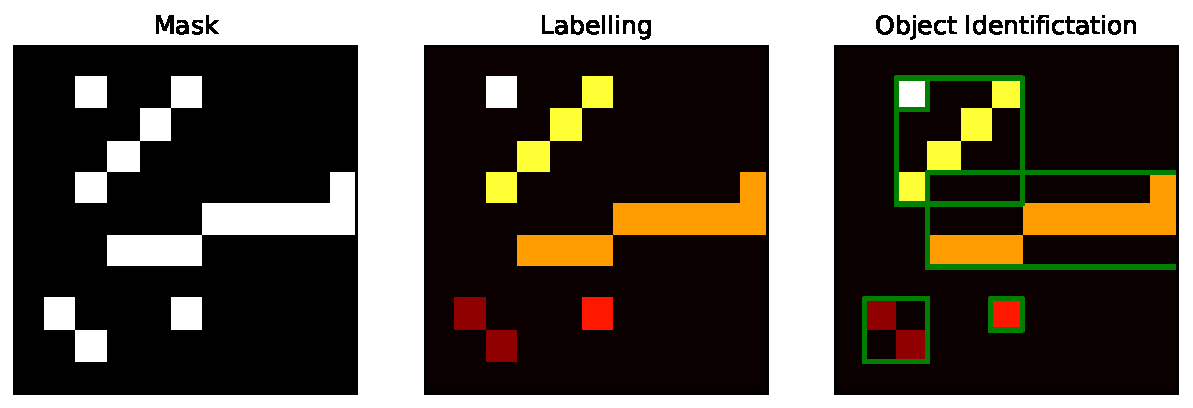
\includegraphics[width=\textwidth]{images/extraction/TrackObs_Objects}
  \caption{Identification of individual connected objects from a cosmic ray mask. The boolean mask (left panel) is used to calculate an integer array for all 8-connected pixels, which are labeled with a unique integer per object (middle panel). Objects are then identified by their labels as rectangular image sections around all pixels with a common label (green boxes in right panel).}
  \label{fig:TrackObs_Objects}
\end{figure}

First, individual objects are identified from the mask. This process is shown in Figure \ref{fig:TrackObs_Objects}. From the boolean mask, a labelling algorithm from the \texttt{scipy} Python distribution is used to assign the same integer value to all neighbouring pixels set to True -- in this case, if they are horizontally, vertically or diagonally adjacent. The labelled array is then used by a \texttt{scipy} object finding algorithm to identify the bounding boxes of all pixels of the same label.

Each TrackObs then contains an array whose rows represent information on one of the objects identified in the above steps. For each track, it lists:
\begin{itemize}
  \item The AL and AC lengths of the bounding box
  \item The location of the track, encoded as the lowest AL and AC value in its bounding box
  \item The sub-image of the track from the signal array, encoded in ADU. Note that this only includes those pixels inside the bounding box with the corresponding label - in the right panel of Fig. \ref{fig:TrackObs_Objects}, the image of the $4 \times 4$ diagonal track in the upper left does not include the single pixel track in its bounding box, which has a different label.
  \item The sum of signal values of the track in electrons, corresponding to the total measured ionizing energy.
  \item The uncertainty of the total ionizing energy, being the square root of the sum of the squares of the individual pixel uncertainties.
\end{itemize}

Each of the following algorithms produces such TrackObs objects, which are saved intermediately as FITS files.




\subsubsection{SM-SIF: Laplacian Edge Detection}
\label{sec:extrSM-SIF}
\begin{figure}
  \centering
  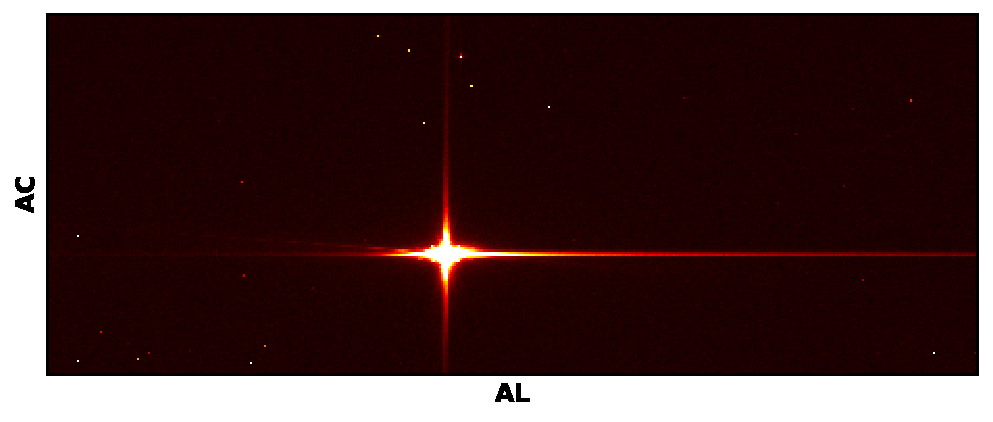
\includegraphics{images/extraction/SM_full_image}
  \caption{An example of a SM-SIF source image. Axis orientation is the standard Gaia convention, with the serial register to the right and readout to the upper right corner. The aspect ratio has not been corrected for pixel geometry and binning.}
  \label{fig:SM_full}
\end{figure}

Figure \ref{fig:SM_full} demonstrates a typical image in the SM-SIF dataset. The image contains a bright star object with a PSF that contains long diffraction spikes and a saturated core. Smaller stars and what appear to be cosmic ray tracks can be detected by bare eye.

To automate the detection of cosmic ray tracks in these images, they must be successfully separated from the imaged astronomical objects. Such algorithms, usually used to remove unwanted cosmic rays, have been developed for earlier ground- and space-based observatories and can be used in to our advantage. For this dataset, we decided to utilize the \textsc{L.A. Cosmic} algorithm described in \cite{Dokkum_cosmics}. Briefly summarized, this algorithm utilizes a variation of Laplacian edge detection to discriminate cosmic ray tracks from stars by their sharp edges, which separates them from the smoother PSFs of stars.

In more detail, the algorithm first convolves a subsampled version of the original image with a derivative filter, which assigns high values to sharp edges. The resulting image is compared with a noise image, calculated by a $5 \times 5$ median filter of the image and including the CCD readout noise. Pixels with a signal-to-noise-ratio above a high threshold are then selected as first candidates for noise pixels, after which a lower threshold is applied to neighbouring pixels. The identified pixels are then masked and the original image is cleaned, replacing the cosmic ray pixels with the median or mean of the surrounding, unmasked pixels. This procedure, starting from the convolution, is applied iteratively until either no more pixels are identified or the maximum number of iterations has been reached.

This analysis utilizes a Python implementation of the \textsc{L.A. Cosmic} algorithm called \textsc{Astro-SCRAPPY} \cite{astroscrappy} for cosmic ray identification.

First attempts at simply applying \textsc{Astro-SCRAPPY} to images like the one in Fig. \ref{fig:SM_full} revealed that the bright stars in most of the SM-SIF images were still falsely detected as cosmics. The reason for this is their saturation of the detector -- see especially the middle panel of Figure \ref{fig:SM_starmask}. The bright star, as it saturates the detector, causes a strong blooming effect, saturating even the pixels read in after those exposed to the bright stars (the image read out direction is to the top). As the panel shows, the resulting pattern has a very sharp gradient, which is picked up by the Laplacian filter and mis-identified as a cosmic.

\begin{figure}
  \centering
  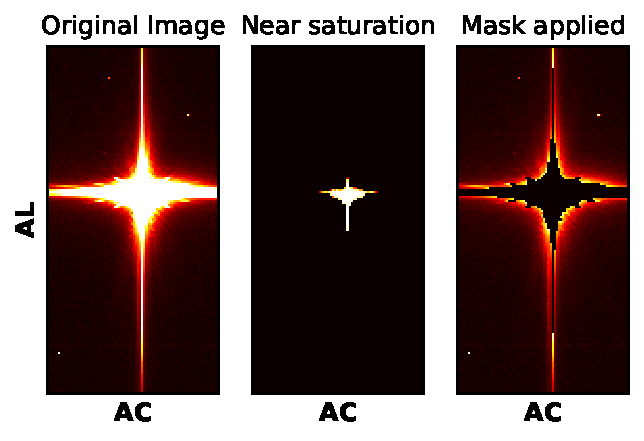
\includegraphics{images/extraction/SM_starmask}
  \caption{Bright stars in SM-SIF and their masking. \textit{Left:} The appearance of the bright star from Fig. \ref{fig:SM_full}. \textit{Middle:} The left panel after applying a high threshold. The bright pixels are fully saturated and show a sharp charge transfer pattern. \textit{Right:} The left panel after applying bright star filtering - the core and a large part of the diffraction spikes are masked.}
  \label{fig:SM_starmask}
\end{figure}

To eliminate these bright star cores and mask their extended field, in which cosmics will disappear under the poisson noise of the star, we apply a simple algorithm before extracting cosmics. Its steps are:
\begin{enumerate}
  \item Object finding: Construct a mask set to 1 for every pixel above a low threshold and apply object labelling to this mask. This step essentially catches all stars and cosmics.
  \item Saturated object identification: Of all objects, select only those that contain at least one pixel at a value of 65535 ADU, the maximum of a 16-bit integer. 
  \item Masking: Add all the objects identified in the previous steps to a mask (set to 1 for invalid pixels). This mask can be forwarded to \textsc{Astro-SCRAPPY}, which supports masked regions and does not use them for cosmic identification.
\end{enumerate}

The results of this algorithm can be seen in the right panel of Fig. \ref{fig:SM_starmask}, where all pixels belonging to the bright star are set to zero. There still remain some parts of the bright star's PSF - these, however, are very close to the bias level and decay smoothly, thus causing no issues.

Using the bright star removal, we then constructed the following algorithm to extract cosmics from SM-SIF observations:
\begin{enumerate}
  \item Read in the image and construct the bright star mask.
  \item Subtract the AL-dependent bias and apply the gain-scale, as \textsc{L.A. Cosmic} requires an image in units of electrons to calculate the Poisson noise.
  \item Apply \textsc{L.A. Cosmic}, which returns the cosmic ray mask and a cleaned image. The values of the cleaned image are calculated by taking the mean of the surrounding, non masked pixels in a $5 \times 5$ pixel area, i.e. for a pixel located at $\left(AL,AC\right)$, the cleaned value is
    \begin{equation}
      \mathrm{Clean}\left(AL,AC\right) = \left( \sum\limits^\mathrm{mask=False}_{\substack{AL-2 \leq i \geq AL+2 \\ AC-2 \leq j \geq AC+2}} \mathrm{Source}\left( i, j \right) \right) \bigg/ \left( \sum\limits^\mathrm{mask=False}_{\substack{AL-2 \leq i \geq AL+2 \\ AC-2 \leq j \geq AC+2}} 1\right)
    \end{equation}
  \item Calculate the signal array as $~\mathrm{Signal}\left(AL, AC\right)= \mathrm{Source}\left(AL, AC\right) - \mathrm{Clean}\left(AL, AC\right)$
  \item Calculate the uncertainty array as the square root of the variance of the signal array, calculated as
    \begin{equation}
      Var\left(AL,AC\right) = \mathrm{Source}\left(AL,AC\right) + \sigma_\mathrm{rn}^2 + \sum\limits^\mathrm{mask=False}_{\substack{AL-2 \leq i \geq AL+2 \\ AC-2 \leq j \geq AC+2}} \frac{\mathrm{Source}\left(i,j\right) + \sigma_\mathrm{rn}^2}{N_\mathrm{mean}\left(AL,AC\right)},
    \end{equation}
    with $\sigma_\mathrm{rn}^2$ denoting the pixel readnoise, and $N_\mathrm{mean}\left(AL,AC\right)$ denoting the number of pixels used to calculate the mean for cleaning this pixel. As one can see from the equation, the noise of the source image has been assumed to be Poissonian noise and readnoise.
  \item Extract tracks from the mask, signal and uncertainty images and save them as a TrackObs, as described above.
    
\end{enumerate}

The parameters used for the \textsc{L.A. Cosmic} algorithm were first selected manually, by applying the extraction algorithm to individual images and viewing the output. Selection criteria were that no stars should be misidentified as cosmic ray tracks, and that cosmic ray tracks should be complete, meaning that a single, long track should result in exactly one identified object.

To verify and further tune the extraction algorithm with regards to the detection efficiency and measurement accuracy, it was necessary to have known input data with which to compare the measured output. To that extent, we utilized a previously developed CCD cosmic ray events simulator called T.A.R.S. (Tools for Astronomical Radiation Simulations) developed at ESTEC \cite{TARS}. The tool simulates the energy deposition of a cosmic ray in a CCD detector along with the charge collection to produce simulated CCD images. The first implementation of the tool was built to simulate Gaia images and was thus suited for this activity.

To test the extraction algorithm, we first prepared an SM observation by cleaning it with \textsc{L.A. Cosmic}, removing any existing cosmics that would be detected by our algorithm. For the source image, we selected a large image without any saturated stars, as these cosmics could not be detected there in any case and we were more interested in 'normal' stars.

We then generated cosmic ray tracks on the image, saving the locations and deposited energies for every simulated cosmic. Afterwards, we ran the extraction algorithm from above and analysed the results by associating each simulated track with the tracks recovered in its image location. Figure \ref{fig:SM_extr_verif} shows two figures of merit for the extraction algorithm: The detection efficiency and the error of the extracted energies with respect to the calculated uncertainty.

The detection efficiency (left panel of Fig. \ref{fig:SM_extr_verif}) shows the number of detected tracks per input track - a value of 1 being a correct detection, a value of 0 being a non-detection and a value greater than one implying that parts of the track could not be identified, leading to multiple detections. The overall number of correctly detected events is greater than 97\,\%.

The error in extracted energies is shown in the left panel of Fig. \ref{fig:SM_extr_verif}, and plots the difference between the measured track energy and the ionizing energy dumped by the simulated cosmic on the detector. For each track, this value is normalized by the uncertainty of the measured energy. A comparison of the resulting histogram with a Gaussian with a standard deviation of 1 shows that the energy measurements are correct within their estimated errors.




\begin{figure}
  \centering
  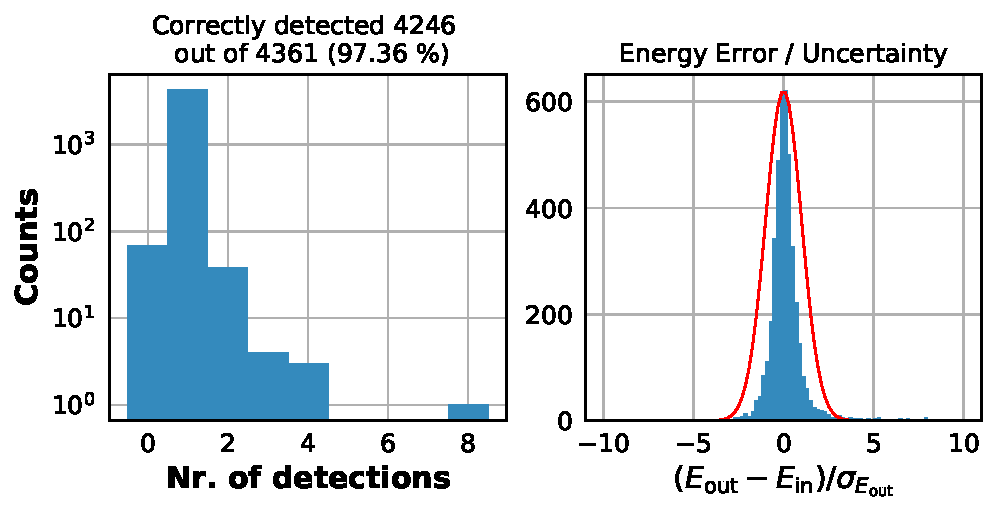
\includegraphics[width=\textwidth]{images/extraction/verification_sm-sif}
    \caption{Figures of merit for the SM-SIF extraction. \textit{Left:} Histogram of the number of associated track detections per input cosmic. A value of 0 is a non-detection, a value of 1 is a correct detection, a value of $>\!1$ means a single cosmic has resulted in multiple detections. \textit{Right:} Histogram of the difference between measured and input track energy per cosmic, normalized by the calculated uncertainty. A Gaussian with a standard deviation of 1 is plotted in red.}
  \label{fig:SM_extr_verif}
\end{figure}


\subsubsection{BAM-OBS: Boxcar filtering / Stacking}
\label{sec:extrBAM-OBS}
\begin{figure}
  \centering
  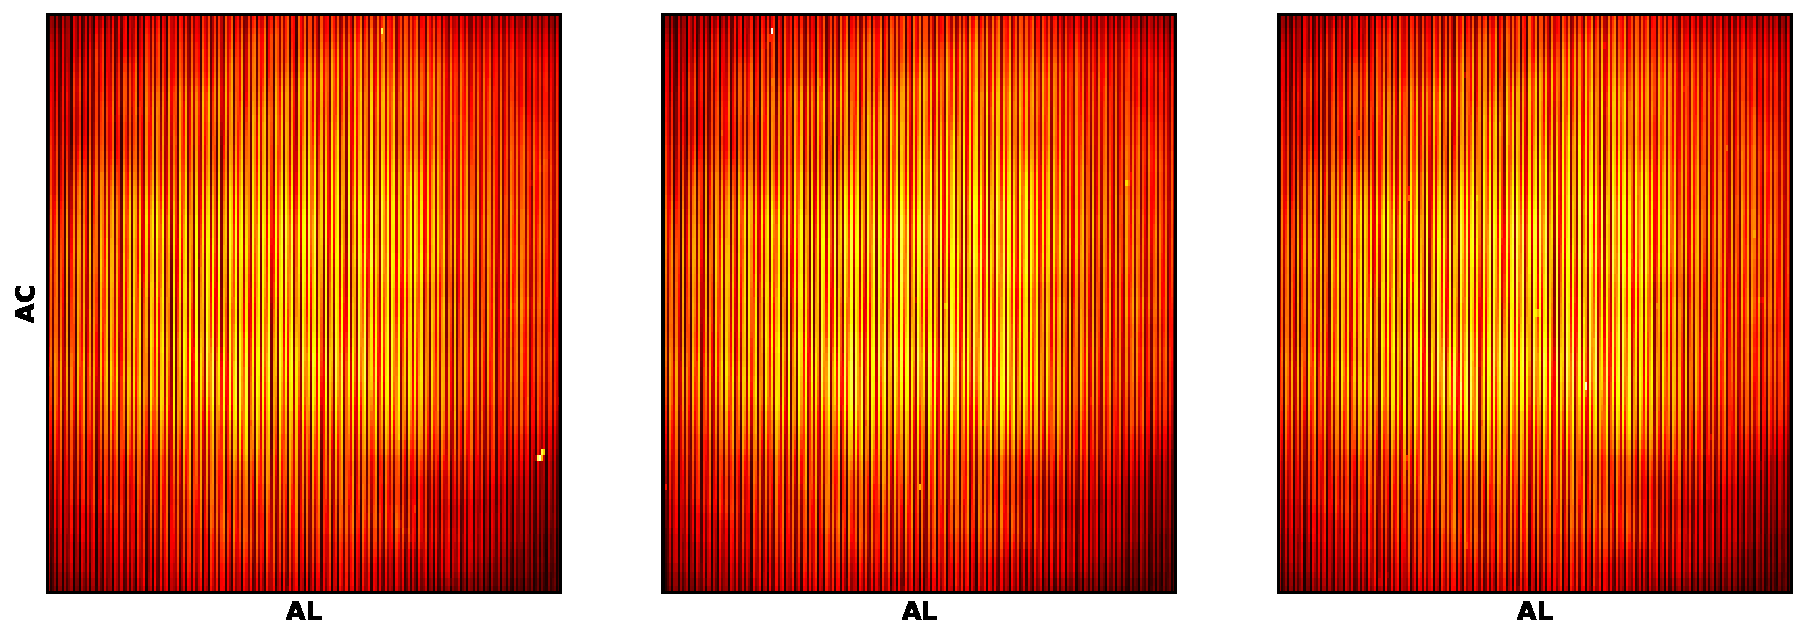
\includegraphics[width=\textwidth]{images/extraction/BAM-OBS_patterns}
  \caption{A series of three BamObservations from FOV 1. The dimensions have been rescaled to the physical dimension of the CCD -- each image pixel represents a $10 \times 120\, \mu m$ (AL $\times$ AC) sample. Individual pixels that deviate from the patterns can be recognized as cosmic ray tracks.}
  \label{fig:BAM_patterns}
\end{figure}

Figure \ref{fig:BAM_patterns} shows a series of observations from FOV 1 of the BAM. The three images were recorded in series (left to right) with an exposure time of about 23 seconds each. It is visibly apparent that the BAM patterns do not significantly between single observations, yet all three images contain pixels deviating from the pattern that only exist in one given image. These spurious pixels are a clear sign of cosmic rays.

\begin{figure}
  \centering
  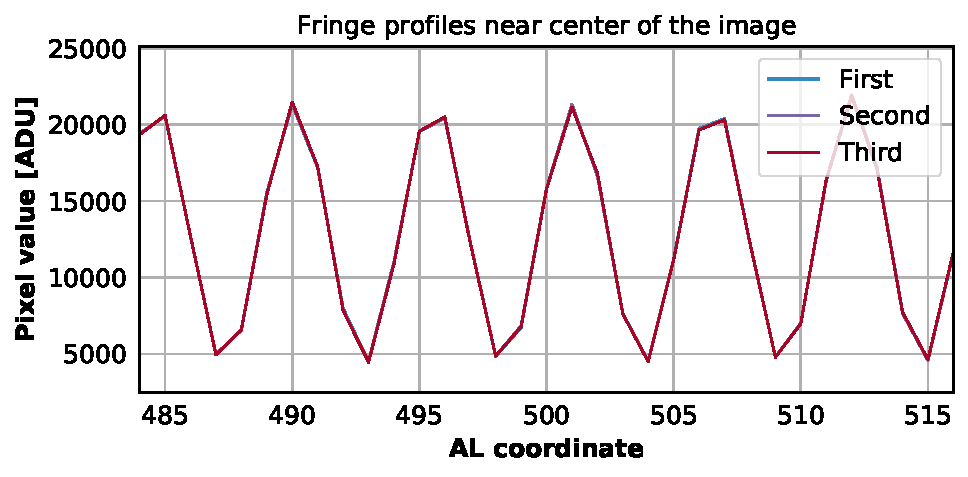
\includegraphics[width=\textwidth]{images/extraction/BAM-OBS_fringes}
  \caption{The ADU values of the three patterns in Fig. \ref{fig:BAM_patterns} plotted along the center of the images in AC across a narrow AL region in the center. The interference pattern is very sharp, with a period of about 5 pixels in AL. The fringes of all three images overlap very closely.}
  \label{fig:BAM_fringes}
\end{figure}

Figure \ref{fig:BAM_fringes} further demonstrates that the interference pattern does not vary aside from Poissonian noise between the three images. It also shows why a simple application of the \textsc{L.A. Cosmic} algorithm to this dataset will immediately fail: The interference patterns themselves are very sharp, with a peak-to-trough distance of about 2 to 3 pixels. The algorithm is totally blinded by the pattern and can not separate it from the cosmics.

For our track extraction algorithm, we exploited the fact that the interference pattern is relatively static. In astronomy, multiple exposures of the same object (assuming constant luminosity) are used to reject the spurious high pixel values caused by cosmic rays -- a similar algorithm is used to reject cosmics in BamObservations when analyzing the pattern. In our case, we can simply do the reverse, and accept pixels that vary significantly stronger than the inherent counting and readout noise as the tracks of cosmic rays.

The concrete algorithm assumes as an input a time-ordered series of BamObservations from a single FOV, and operates on a range of observations, which we refer to as a BoxCar. To create a good estimate of the pattern across a period of time where it does not vary, we chose to use a total of 7 images at once - a central image for cosmic ray extraction and the three images recorded immediately after and before. The extraction algorithm works as follows.

\begin{enumerate}
  \item Construct the BoxCar: Read the first 7 BamObservations -- applying the electron conversion gain -- into a three dimensional array with the indices $t$, $AL$ and $AC$ - with $t \in [1,\cdots,7]$ ($t = 3$ being the central observation), and $AL$ and $AC$ denoting the image dimensions.
  \item Sigma-clipping: Compute the median and standard deviation across time and mark all the pixels whose difference to the median exceeds a chosen threshold - these are likely cosmics, and will not be used to calculate the pattern.
  \item Calculate a two-dimensional image array of the pattern, by taking the mean across time without using the sigma-clipped pixels, e.g.
\begin{equation}
  \mathrm{Pattern}\left( AL,AC \right) = \left( \sum\limits_{t~\mathrm{not~clipped}} \mathrm{BoxCar}\left( t, AL, AC \right) \right) \bigg/ \left( \sum\limits_{t~\mathrm{not~clipped}} 1\right).
\end{equation}
  \item Calculate the signal array by subtracting the Pattern from the central array in the BoxCar, e.g.
\begin{equation}
  \mathrm{Signal}\left( AL,AC \right) = \mathrm{BoxCar}\left(t=3,AL,AC \right) - \mathrm{Pattern}\left( AL,AC \right).
\end{equation}
  \item Calculate the uncertainty array as the square root of the variance of the signal array, calculated as
    \begin{equation}
      Var\left(AL,AC\right) = \mathrm{BoxCar}\left(t=3,AL,AC\right) + \sigma_\mathrm{rn}^2 + \sum\limits_{t~\mathrm{not~clipped}} \frac{\mathrm{Boxcar}\left(t,AL,AC\right) + \sigma_\mathrm{rn}^2}{N_\mathrm{mean}\left(AL,AC\right)},
    \end{equation}
  with $\sigma_\mathrm{rn}^2$ denoting the pixel readnoise, and $N_\mathrm{mean}\left(AL,AC\right)$ denoting the number of pixels in the BoxCar that have not been rejected by sigma clipping at this $\left(AL,AC  \right)$ pair. As one can see from the equation, the noise of the BamObservations has been assumed to be Poissonian noise and readnoise.
  \item Create the cosmic mask: Divide the signal array by the uncertainty array and create the boolean mask array, set to true where the signal/uncertainty ratio is greater than a threshold $f$. Due to the strong photon background, some cosmic pixels are missed in this step. We attempt to mitigate this by investigating all the pixels that neighbour the previously masked pixels, found via binary dilation, and applying for them a signal/uncertainty threshold of $r_\mathrm{Neighbour}*f$, adding the pixels that satisfy this condition to the mask as well.
  \item \label{item:connectAlg} Apply a track connection algorithm: Even after the previous step, visually apparent long cosmic ray tracks still remain separated - refer to the left panel of Figure \ref{fig:BAM_connection} for an illustration. Tracks that are oriented in the AL direction see a strongly variable photon background, seen as fluctuations in the uncertainty array. These pixels are less likely to be detected by the thresholding of before. Especially towards the center of the image, where the pattern amplitude is very high, this leads to a single, long cosmic being detected as multiple short cosmics in the troughs of the interference pattern, which eventually leads to an overestimation of the cosmic ray rate.

    In an attempt to correct for this track separation, we implemented a track connection algorithm: We first apply to the mask an 8-connected binary dilation followed by a 4-connected binary erosion (this is a variant on binary closing, which uses the same structuring elements for the dilation and erosion instead), illustrated in the middle and right panels of Fig. \ref{fig:BAM_connection}. As the Figure shows, this marks several pixels of interest that may connect the separated objects.

    We then examine each of the newly merged tracks, which are identified by the standard labelling algorithm. For each of the tracks, we first calculate the mean of the previously identified signal pixels of this track, $m_\mathrm{Object}$. Assuming that a cosmic ray creating a long track should have a constant energy deposition per path length, we examine each of the candidate pixels (at the location $\left(AL,AC\right)$), checking for the condition
    \begin{equation}
      \lvert Signal\left( AL,AC \right) - m_\mathrm{Object}\rvert > cfac * \sqrt{Var\left( AL,AC \right)},
    \end{equation}
    with $cfac$ being an algorithm parameter. The above equation checks whether the signal value of the candidate pixel is sufficiently close to the value of the other pixels in this object. If a pixel satisfies the condition, it is added to the pixel mask. 
  \item Extract tracks from the mask, signal and uncertainty images and save them as a TrackObs, as in SM-SIF and described above.
  \item Update BoxCar: Read in the next BamObservation and replace the oldest pattern in the BoxCar with it -- the BoxCar is utilized as a FIFO, in this case. We then update the central pixel index and repeat starting step 2 until all BamObservations have been processed.
\end{enumerate}

\begin{figure}
  \centering
  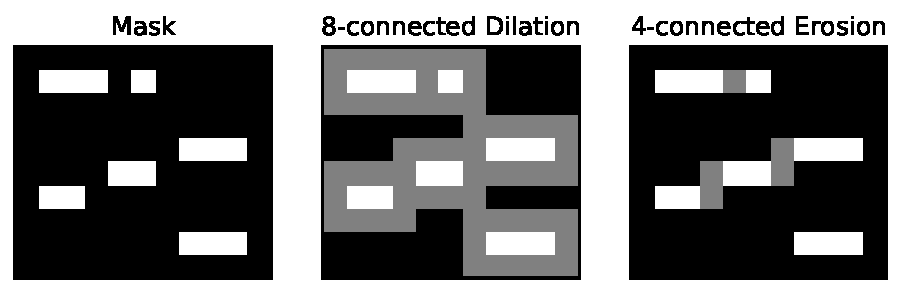
\includegraphics{images/extraction/BAM-OBS_connection}
  \caption{Illustration of the track connection algorithm used for this dataset. \textit{Left:} An example of a cosmic ray mask where ray tracks oriented in the AL direction have not been fully identified. \textit{Middle:} Application of 8-connected binary dilation to the mask - the added pixels are shown in gray. \textit{Right:} Additional application of 4-connected binary erosion, shown in the gray pixels, which are examined by the connection algorithm.}
  \label{fig:BAM_connection}
\end{figure}

As we did for the SM-SIF extraction, we also tested the BAM-OBS extraction algorithm using the T.A.R.S. package. In the case of BAM-OBS, we first created a series of fake BAM patterns by calculating a running median over a set of 100 successive BamObservations. Concretely, we took for every observation the four preceding and four next observation and calculated the median image of these observations. Afterwards, we added Poissonian counting noise to each image.

We then added simulated cosmic ray tracks to all images and ran the extraction algorithm over the list of observations. As in the SM-SIF verification, we associated each input track with the detected tracks in its image location. As in the previous verification, Figure \ref{fig:BAM-OBS_extr_verif} shows the detection efficiency and normed energy error for the BAM-OBS extraction, once again returning consistent values for both. Note that these plots show results for FOV 2, whose interference pattern has a higher intensity and thus noise.

\begin{figure}
  \centering
    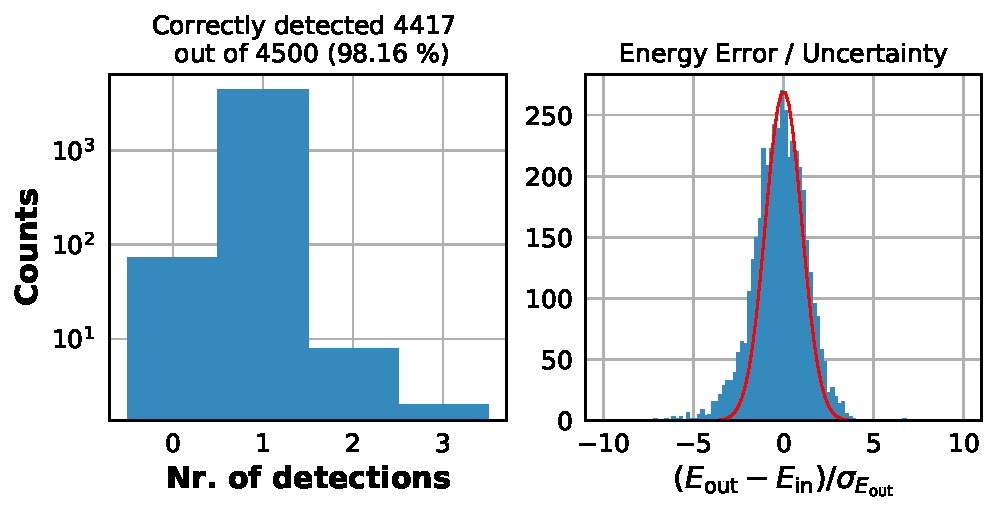
\includegraphics[width=\textwidth]{images/extraction/verification_bam-obs_mended}
    \caption{Figures of merit for the BAM-OBS extraction, as in Fig. \ref{fig:SM_extr_verif}.}
  \label{fig:BAM-OBS_extr_verif}
\end{figure}

To justify the use of the connection algorithm (step \ref{item:connectAlg} above), Fig. \ref{fig:BAM-OBS_nomend_extr_verif} shows the figures of merit for the same input data as Fig. \ref{fig:BAM-OBS_extr_verif} when the connection algorithm is not used. While the measured energies don't differ significantly, the number of input tracks recognised as multiple output tracks is lowered by the connection algorithm.

\begin{figure}
  \centering
    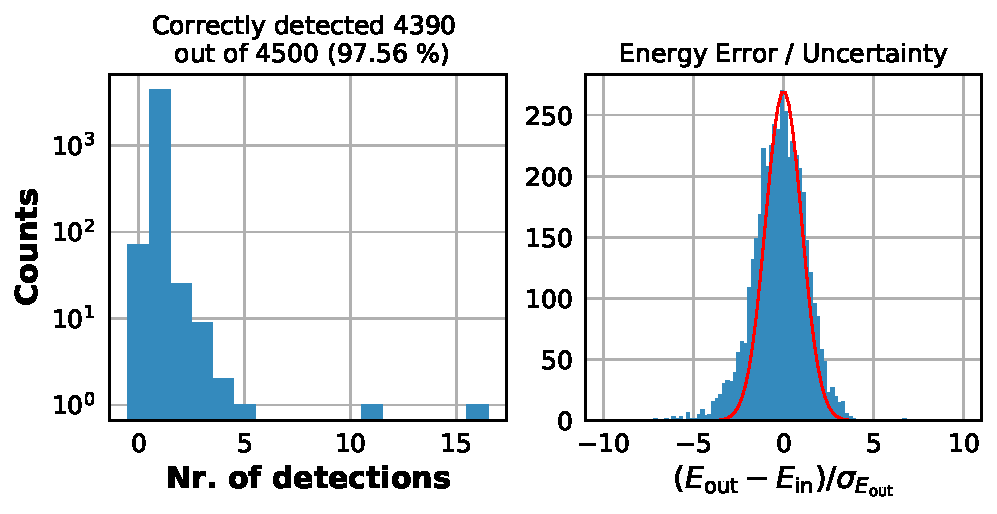
\includegraphics[width=\textwidth]{images/extraction/verification_bam-obs_old}
    \caption{Figures of merit for the BAM-OBS extraction without the track connection algorithm. Compared to Fig. \ref{fig:BAM-OBS_extr_verif}, individual cosmics are more likely to be identified as multiple tracks.}
  \label{fig:BAM-OBS_nomend_extr_verif}
\end{figure}


\subsubsection{BAM-SIF: Thresholding}
\label{sec:extrBAM-SIF}
\begin{figure}
  \centering
  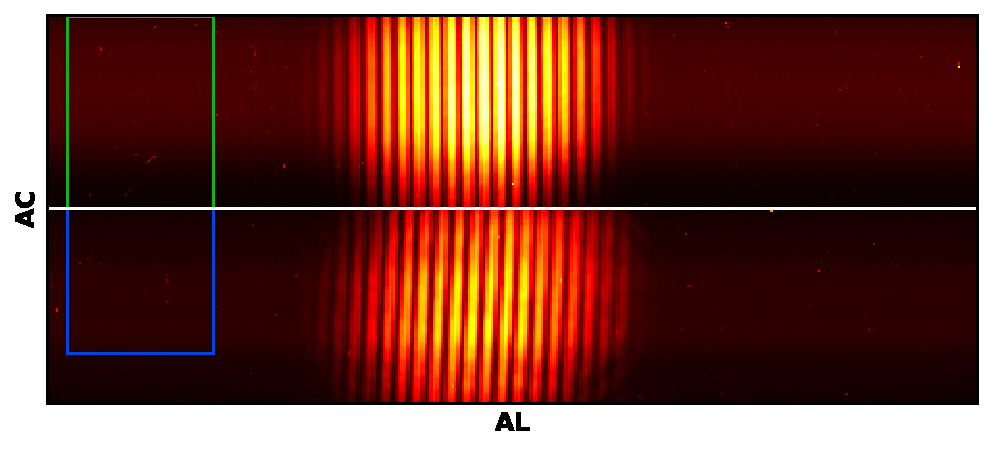
\includegraphics{images/extraction/BAM-SIF_full_image}
  \caption{An example of a BAM-SIF source image, which has been rescaled to the physical CCD dimensions. The top half of the image shows the AC region of FOV 2, the bottom half that of FOV 1. The off-pattern regions in green and blue boxes are used for cosmic extraction.}
  \label{fig:BAM-SIF_full}
\end{figure}

Figure \ref{fig:BAM-SIF_full} depicts an example for a BAM-SIF image used in this extraction. These images both contain the interference pattern in the BAM-OBS images, as well as off-pattern regions showing the TDI footprint of the pattern, which is only AC-dependent. These images are much less frequently sampled than the BAM-OBS images -- usually a handful of images twice per week -- which is why they are not very useful for the purpose of particle monitors. However, the off-pattern regions offer a good opportunity to extract cosmics from the BAM chip with a much lower and simpler background than that of BAM-OBS, allowing us to examine the effect the pattern has on the above extraction.

As this dataset is very attractive for cosmic ray extraction, it has been used before for cosmic ray studies, see \cite{GAIA-DE-TN-ESAC-RKO-033}. This algorithm builds on the previous extraction, merging it into the TrackObs-based files approach utilized here.

For the extraction of cosmics, we utilize the two regions outlined in blue and green boxes in Fig. \ref{fig:BAM-SIF_full}. A smaller region in AC has been selected for the FOV 1 region - the ignored region has shown a high stray light contamination, which causes mis-identifications.

The extraction algorithm for this dataset is then (for each region seperately):
\begin{enumerate}
  \item Read in the image and apply the gain scale.
  \item Determine the AC-dependent TDI background: Take the 99 columns with the highest AL value (to the left in Fig. \ref{fig:BAM-SIF_full}) and remove the outliers -- for each column within, discard the highest and lowest 25\,\% of pixel values to remove cosmics. Then, calculate the mean and standard deviation of the remaining image pixels for each line. The output are two one-dimensional arrays of the AC-dependent TDI background and its standard deviation.

    The removal of the TDI background is demonstrated in Figure \ref{fig:BAM-SIF_background}
  \item Calculate the signal and variance arrays as
    \begin{equation}
      Signal\left( AL,AC \right) = Source\left( AL,AC \right) - Background\left(AC \right)
    \end{equation}
    and
    \begin{equation}
      Var\left( AL,AC \right) = Source\left( AL,AC \right) + \sigma_\mathrm{rn} + \sigma_\mathrm{Background},
    \end{equation}
    with $\sigma_\mathrm{rn}$ being the readnoise and once again assuming Poisson noise in the source array. The uncertainty array is then the square root of the variance array.
  \item Construct the mask array in exactly the same way as for BAM-OBS, including the track connection. While this should not be necessary here, we want to have as similar as possible algorithms for BAM-OBS and BAM-SIF, to see the effect of the pattern.
  \item Extract tracks from the mask, signal and uncertainty images and save them as a TrackObs, as in the algorithms above.
\end{enumerate}

\begin{figure}
  \centering
  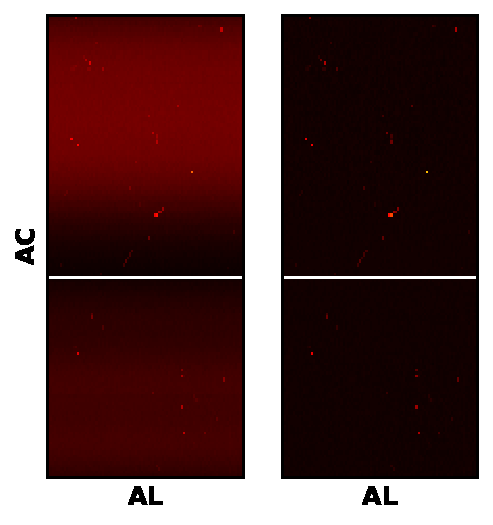
\includegraphics{images/extraction/BAM-SIF_background}
  \caption{\textit{Left:} The two extraction regions from Fig. \ref{fig:BAM-SIF_full}. \textit{Right:} The same image with the TDI backround removed, leaving only cosmic ray tracks.}
  \label{fig:BAM-SIF_background}
\end{figure}

All steps until the calculation of the signal are the same as in \cite{GAIA-DE-TN-ESAC-RKO-033}, which only returned the signal images.

As in both previous algorithms, we once again verified the BAM-SIF extraction against simulated cosmics. In this case, a fake TDI background was obtained by removing outliers from a BAM-SIF observation. A background image is then randomly sampled from the extracted background. Afterwards, simulated cosmic ray tracks are added on top of the produced image and extracted via the BAM-SIF algorithm. The figures of merit obtained in the same way as before are plotted in Figure \ref{fig:BAM-SIF_extr_verif}, showing a very good detection efficiency and energy errors within the bounds expected from the calculated uncertainties.
\begin{figure}
  \centering
    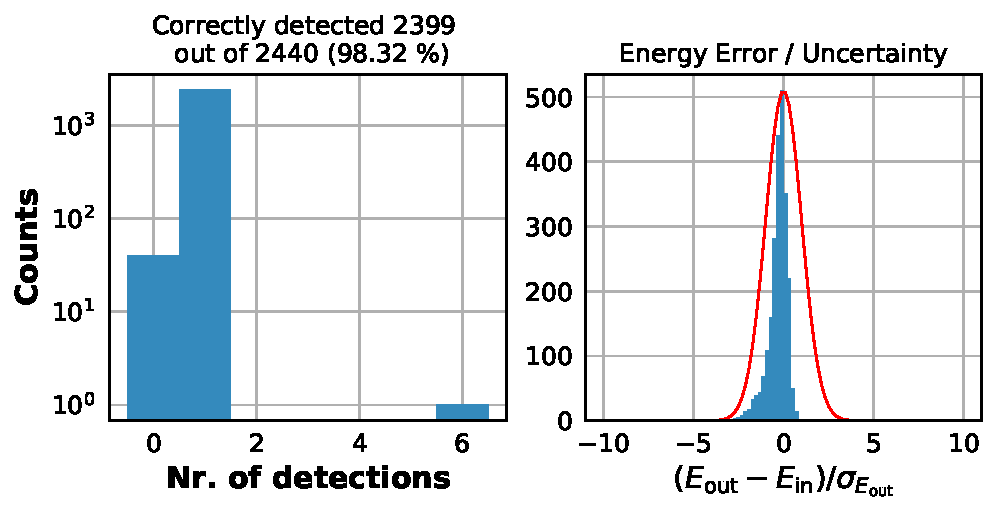
\includegraphics[width=\textwidth]{images/extraction/verification_bam-sif}
    \caption{Figures of merit for the BAM-SIF extraction, as in Fig. \ref{fig:SM_extr_verif}.}
  \label{fig:BAM-SIF_extr_verif}
\end{figure}


\subsubsection{Extraction Pipeline}

Having specified the extraction of cosmic ray tracks from the images themselves, we now describe the  extraction pipelines used to systematically retrieve the image data files from the Gaia Main Database in order to produce and save TrackObs from them.

\paragraph{SM-SIF and BAM-SIF}
\paragraph{BAM-OBS}
\subsection{Post-Processing}
\label{sec:postprocessing}
For the final data product described in Section \ref{sec:CosObsModel}, we derive additional data from the raw extracted tracks in a TrackObs. The algorithms for deriving these are outlined in this section
\subsubsection{Observed Flux}

One of the first -- and most simple -- data products that can be derived from a TrackObs is the flux measured per observation. The calculation of a flux is in this case very simple: Given an exposed CCD area $A_\mathrm{exp}$ and exposure time $T_\mathrm{exp}$ the flux is simply calculated as

\begin{equation}
  F = \frac{\mathrm{Counts}}{A_\mathrm{exp} \cdot T_\mathrm{exp}}
\end{equation}

In the following, we determine these values for SM-SIF and BAM observations, whose computation are not trivial due to the use of TDI (and in the latter case, staring) observations and the size of the used AL readout windows relative to the physical CCD size.

For our calculations: A Gaia CCD is segmented into 4500 pixels in AL direction and 1980 pixels in AC direction - of these, 14 pixels are in the pre-scan region and not used. Pixels are $10 \times 30\, \mathrm{\mu m}$ (AL $\times$ AC) and TDI transfer time is $T_\mathrm{TDI} = 0.9828\, \mathrm{ms/pixel}$, so the effective CCD exposure time is 4.4226\,s.

\paragraph{SM-SIF \\}

The readout of the SM-SIF images are a continuous readout of the signal acquired from TDI (see also Fig. \ref{fig:SM_Acq}). To avoid saturation from bright stars, Gate 12 is permanently activated, leading to a readout of only the last 2900 CCD lines in AL. Pixels are then binned to a factor of 2 in both AL and AC.

\begin{figure}[h]
  \centering
  {\Huge TIKZ PLACEHOLDER}
%  \begin{tikzpicture}[scale=1]
%
%    % Part 1: A physical image of the CCD, with gate 12
%    \node(scope1){
%      \begin{tikzpicture} 
%        \draw[thick] (0,0) rectangle (1.5,3); % box
%        \draw[thick,blue] (0.53,-0.2) -- (0.53,3.2); % Line for gate 12
%        \draw[thick,red] (1.5,0) -- (1.5,3); % Readout
%        \draw[thick,-{Latex[length=8pt]}] (0.6,1.5) to (1.4,1.5);
%        
%        \node[blue] at (0.3,3.4) {Gate 12}; % Marker for gate 12
%        \node[red] at (1.8,-0.3) {Readout}; % Marker for Readout
%        \node at (1,1.8) {TDI}; % Marker for Readout
%
%
%      \end{tikzpicture} 
%    };
%
%    % Part 2: The output image
%    \node[at={($(scope1.east)+(.1cm,0)$)},anchor=west](scope2){
%      \begin{tikzpicture} 
%        % the box around it
%        \draw[thick, fill] (0,0) rectangle (5,3);
%
%        % A few stars
%        \node[star,star points=4, star point height=.7cm, draw, fill=white] at (1,1) {};
%        \node[star,star points=4, star point height=.1cm, draw, fill=white] at (4,2) {};
%        \node[star,star points=4, star point height=.1cm, draw, fill=white] at (.5,2.5) {};
%
%        % And some cosmics
%        \draw[thick,white] (3.5,2) -- (3,1.5) (1.2,2.5) -- (1.3,2)
%                           (4,0.2) -- (4.5,0.3);
%      \end{tikzpicture} 
%    };
%
%    % a big arrow between them
%    \draw[red, ultra thick,-{Stealth[length=.5cm, width=.7cm]}] ($(scope1.east) + (-1cm,0)$)  to ($(scope2.west)$);
%
%  \end{tikzpicture}
  \caption{Scheme of an SM acquisition. The CCD area of each chip after Gate 12 is continuously read out via TDI (left). The resulting image (right) has the same dimension in AC but a dimension in AL dependent on the duration of the readout.}
  \label{fig:SM_Acq}
\end{figure}


For clarity in notation, I will, from now on, use the following terms:
\begin{itemize}
  \item A \textbf{CCD pixel} refers to a physical pixel on the actual CCD - i.e. one physical unit of $10 \times 30\, \mathrm{\mu m}$
  \item An \textbf{image pixel} refers to a pixel in the image recorded after the TDI scan. While it still carries spatial information in AC, its AL information is a result of the integration over the sampled region in AL - it encodes time and location. Thus, an image pixel does not correspond to a single physical pixel, but rather the history of an entire AL line during TDI.
\end{itemize}


The resulting image, then, consists of 983 image pixels in AC and a variable number $N_\mathrm{AL}$ of image pixels in AL - depending on the time over which data has been recorded (which is $T_\mathrm{rec} = T_\mathrm{TDI} \cdot 2 N_\mathrm{AL}$).

From a physical pixel perspective, each CCD pixel has been exposed for the time $T_\mathrm{rec}$, with the information of individual exposures spread over different image pixels in AL. The exposed area corresponds to that of 2900 $\times$ 1966 physical pixels.

From an image pixel perspective, each pixel has been exposed for exactly $T_\mathrm{TDI} \cdot 2900$, regardless of $N_\mathrm{AL}$. The physical area of each image pixel corresponds to that of 4 physical pixels, due to binning.

As one can tell from the above, the physical perspective has a lower number of pixels, but a higher exposure time per pixel (assuming $2 N_\mathrm{AL} > 2900$). The image perspective has more pixels, but lower exposure times. Irregardless of the perspective, the product $A_\mathrm{exp} \cdot T_\mathrm{exp}$ -- which is of interest for computing fluxes -- is always the same, being

\begin{align}
  \mathrm{Physical: }~ A_\mathrm{exp} \cdot T_\mathrm{exp} &= \left(2900 \cdot 1966 \cdot 10\,\mu m \cdot 30\,\mu m\right) \cdot \left( T_\mathrm{TDI} \cdot 2 N_\mathrm{AL} \right)\\
  \mathrm{Image: }~ A_\mathrm{exp} \cdot T_\mathrm{exp} &= \left(N_\mathrm{AL} \cdot 893 \cdot 4 \cdot 10\,\mu m \cdot 30\,\mu m\right) \cdot \left( T_\mathrm{TDI} \cdot 2900 \right)\\
  &= 33.62 ~ \left(\frac{N_\mathrm{AL}}{1000}\right)\,\mathrm{cm^{2}\,s}
\end{align}

Going forward, we will use the image perspective, as it is consistent with prior studies of the BAM image and more useful for the next section. It is also, as we'll see later, easier to treat masked pixels. Nevertheless, for the calculation of fluxes, both perspectives are equivalent.

\paragraph{BAM-OBS and BAM-SIF}

For the BamObservations, pixels are binned by a factor of 4 in AC and not binned at all in AL.

The determination of an exposure time in both pictures for the BamObservations is complicated by the fact that it is not only a TDI observation, but also contains a period of staring. Normally, the BAM CCD is operated in TDI mode, in the same way as the SM CCD. To record the interference pattern, an exception is made -- for an integration time of 19\,s, the shifting of charges is stopped, and the chip operates in a kind of staring mode. In nominal BamObservations, data is then only aquired from sub-regions of the CCD that have been illuminated by the BAM pattern. BAM-SIF images use the entire CCD in AL direction along a restricted AC range.

\begin{figure}[h]
  \centering
  {\Huge TIKZ PLACEHOLDER}
%  \begin{tikzpicture}[scale=1]
%%    % Begin with one node ecompassing everything
%%    \node[anchor=south west,inner sep=0,minimum width=\textwidth, minimum height=4cm] (image) at (0,0) {};
%%      \begin{scope}[x={(image.south east)},y={(image.north west)}]
%%
%%      \end{scope}
%
%    % Draw five scopes, each corresponding to one box
%    % Each box should also contain the bam patterns!
%
%    % Box 1: Create the readout windows
%    \node(scope1){
%      \begin{tikzpicture} 
%        \node at (-0.3,3) {a)};
%        \draw[thick] (0,0) rectangle (1.5,3); % box
%        \draw[red,opacity=0.5, fill] (0.75,2) circle (0.2);   % pattern1
%        \draw[red,opacity=0.5, fill] (0.75,1) circle (0.2);   % pattern1
%
%        % readout windows
%        \draw[thick,darkgreen,dashed] (0,1.7) -- (-0.3,1.7) -- (-0.3,2.3) -- (0,2.3);
%        \draw[thick,darkgreen] (0,1.7) -- (0.3,1.7) -- (0.3,2.3) -- (0,2.3);
%
%        \draw[thick,blue,dashed] (0,0.7) -- (-0.3,0.7) -- (-0.3,1.3) -- (0,1.3);
%        \draw[thick,blue] (0,0.7) -- (0.3,0.7) -- (0.3,1.3) -- (0,1.3);
%      \end{tikzpicture} 
%    };
%
%    % Box 2: Move the readout windows
%    \node[at={($(scope1.east)+(.6cm,0)$)},anchor=west](scope2){
%      \begin{tikzpicture} 
%        \node at (-0.6,3) {b)};
%        \draw[thick] (0,0) rectangle (1.5,3);
%        \draw[red,opacity=0.5, fill] (0.75,2) circle (0.2);   % pattern1
%        \draw[red,opacity=0.5, fill] (0.75,1) circle (0.2);   % pattern1
%
%        % readout windows
%        \draw[thick,darkgreen] (0.1,1.7) rectangle (0.7,2.3);
%        \draw[thick,blue] (0.1,0.7) rectangle (0.7,1.3);
%      \end{tikzpicture} 
%    };
%
%    % Box 3: Stare
%    \node[at={($(scope2.east)+(.6cm,0)$)},anchor=west](scope3){
%      \begin{tikzpicture} 
%        \node at (-0.6,3) {c)};
%        \draw[thick] (0,0) rectangle (1.5,3);
%        \draw[red,opacity=0.5, fill] (0.75,2) circle (0.2);   % pattern1
%        \draw[red,opacity=0.5, fill] (0.75,1) circle (0.2);   % pattern1
%
%        % readout windows
%        \draw[thick,darkgreen] (0.45,1.7) rectangle (1.05,2.3);
%        \draw[thick,blue] (0.45,0.7) rectangle (1.05,1.3);
%
%      \end{tikzpicture} 
%    };
%
%    % Box 4: Move again
%    \node[at={($(scope3.east)+(.6cm,0)$)},anchor=west](scope4){
%      \begin{tikzpicture} 
%        \node at (-0.6,3) {d)};
%        \draw[thick] (0,0) rectangle (1.5,3);
%        \draw[red,opacity=0.5, fill] (0.75,2) circle (0.2);   % pattern1
%        \draw[red,opacity=0.5, fill] (0.75,1) circle (0.2);   % pattern1
%
%        % readout windows
%        \draw[thick,darkgreen] (0.8,1.7) rectangle (1.4,2.3);
%        \draw[thick,blue] (0.8,0.7) rectangle (1.4,1.3);
%
%      \end{tikzpicture} 
%    };
%
%    % Box 5: Readout 
%    \node[at={($(scope4.east)+(.6cm,0)$)},anchor=west](scope5){
%      \begin{tikzpicture} 
%        \node at (-0.6,3) {e)};
%        \draw[thick] (0,0) rectangle (1.5,3);
%        \draw[red,opacity=0.5, fill] (0.75,2) circle (0.2);   % pattern1
%        \draw[red,opacity=0.5, fill] (0.75,1) circle (0.2);   % pattern1
%
%        % readout windows
%        \draw[thick,darkgreen,dashed] (1.5,1.7) -- (1.8,1.7) -- (1.8,2.3) -- (1.5,2.3);
%        \draw[thick,darkgreen] (1.5,1.7) -- (1.2,1.7) -- (1.2,2.3) -- (1.5,2.3);
%
%        \draw[thick,blue,dashed] (1.5,0.7) -- (1.8,0.7) -- (1.8,1.3) -- (1.5,1.3);
%        \draw[thick,blue] (1.5,0.7) -- (1.2,0.7) -- (1.2,1.3) -- (1.5,1.3);
%
%      \end{tikzpicture} 
%    };
%
%  \end{tikzpicture}
  \caption{Readout scheme for a BAM pattern in BAM-OBS. BAM fringe patterns are outlined as red circles. a) Create the readout windows. b) Move the readout windows via TDI. c) Stare observation -- charges are not shifted. d) Move readout windows via TDI. e) Readout, recording only contents of windows.}
  \label{fig:BAM_Acq}
\end{figure}

The observation principle and the effect on imaging particle tracks is shown in Fig. \ref{fig:BAM_Acq}. Effectively, data is collected from two windows, outlined in green and blue. These two windows have an unbinned length of 1000 in AL and 320 in AC each. They first move across the chip, stay in place during the staring, and then move again to the readout register.

In BAM-SIF observations, we can make a similar estimation of the readout window sizes, although the image dimensions are variable. We will from now on use two values $N_\mathrm{AL}$ and $N_\mathrm{AC}$ to refer to the binned image dimensions of the result image. The used unbinned lengths are then $N_\mathrm{AL}$ and $4\, N_\mathrm{AC}$, respectively -- for reference, a nominal BamObservation has $N_\mathrm{AL} = 1000$ and $N_\mathrm{AC} = 80$

The exposure can once again be viewed in two pictures, the physical pixel and image pixel based ones. In the former, it is easy to see that the entire region both readout windows cross are exposed -- the exposed area is 4500 $\times$ $4\, N_\mathrm{AC}$ pixels (AL $\times$ AC) per pattern. The exposure time, however, is more complex: First, the entire exposed region is exposed for $N_\mathrm{AL} \times T_\mathrm{TDI}$, due to the movement of the readout windows across the chip. Additionally, the region used for staring is observed for a further 19 s. The exposure time is, as such, AL-dependent.

In the image picture, the calculation is much easier. Viewing each readout window as a physical unit, the exposed area per window is simply $N_\mathrm{AL}$ $\times$ $4\, N_\mathrm{AC}$ pixels. The exposure time is simply the TDI transfer time across the whole chip plus the staring time.

The product of exposed area and exposure time, which is of interest for flux determination, is in both pictures (per readout window)

\begin{align}
  \mathrm{Physical: }~ A_\mathrm{exp} \cdot T_\mathrm{exp} = &\left(4500 \cdot 10\,\mu m \cdot 4\, N_\mathrm{AC} \cdot 30\,\mu m \right) \cdot \left( N_\mathrm{AL}\ \cdot T_\mathrm{TDI} \right) \\+ &\left( N_\mathrm{AL} \cdot 10\,\mu m \cdot 4\, N_\mathrm{AC} \cdot 30\,\mu m\right) \cdot \left( 19\,s \right)\\
  \mathrm{Image: }~ A_\mathrm{exp} \cdot T_\mathrm{exp} = &\left( N_\mathrm{AL} \cdot 10\,\mu m \cdot 4\, N_\mathrm{AC} \cdot 30\,\mu m\right) \cdot \left(4500\, T_\mathrm{TDI} + 19\,s \right)\\
  = &22.49\,\mathrm{cm^{2}\,s} ~~~\mathrm{(for~BAM\!\!-\!\!OBS)}.
\end{align}

As the computation is more simple in the image picture, we will from now on use this picture.

\paragraph{Masked Pixels\\}

In both SM and BAM images, some image pixels can not be used for the determination of cosmics. In the SM, these pixels are mostly caused by the bright star masking algorithm. For the BAM, charge overflow effects can be caused by a high energy cosmics coincident with an interference fringe, fully saturating the pixel and causing errors in the readout of several following pixels.

Correcting the exposed area for these masked pixels is very easy in the image picture, as we simply discard these pixels, meaning one can calculate the exposed area using

\begin{equation}
  A_\mathrm{exp} = (N_\mathrm{tot} - N_\mathrm{mask}) \cdot b_\mathrm{AL} \cdot b_\mathrm{AC} \cdot 10 \cdot 30 \, \mu m^{2}
\end{equation}

With $N_\mathrm{tot}$ being the total number of image pixels, $N_\mathrm{mask}$ being the number of masked pixels and $b_\mathrm{AL}$ and $b_\mathrm{AC}$ being the binning factor in AL and AC, respectively.


\subsubsection{Track Geometries}
For particle tracks that pass through multiple pixels, it is possible to estimate the entrance angle of a cosmic into a CCD with respect to the FPA and the length of the path of the particle through the chip. For a selected subset of tracks, this was attempted in this dataset using either simple estimates or a fitting technique.

\begin{figure}
  \centering
  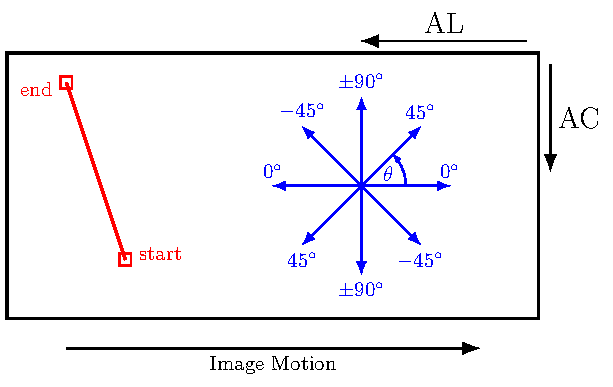
\includegraphics{images/postprocessing/theta_sketch}
  \caption{Definition of the track angle $\theta$ in the standard Gaia CCD reference system. The red line on the left shows an example track, whose start is always defined as the end-point at the lower AL-coordinate. The blue compass rose shows the angle corresponding to different track orientations.}
  \label{fig:theta_sketch}
\end{figure}
Figure \ref{fig:theta_sketch} shows the definition of the angle $\theta$ used in this analysis. It is obtained via the slope of a line describing the cosmic ray track in an (AL,AC) coordinate system, e.g. 
\begin{equation}
  \theta = \tan^{-1} \left( \frac{AC_\mathrm{start} - AC_\mathrm{end}}{AL_\mathrm{start} - AL_\mathrm{end}} \right) [^{\circ}],
  \label{eq:theta_def}
\end{equation}

where the starting point of a track is always defined to be its edge point at the lower AL value. We have made this choice because we do not determine at which of the edge points of a track the cosmic entered and exited the CCD. As such, $\theta$ is defined in a range of $\left[ -90^{\circ}, 90^{\circ} \right]$, with $0^{\circ}$ corresponding to a track completely along the AL axis, $\pm 90 ^{\circ}$ being oriented in the AC direction.

For a track that is one-dimensional, meaning that all its signal pixels are in one line or column, the angle and track length are constrained and can be estimated with a simple algorithm, outlined in Figure \ref{fig:1D_angle}. The particle trajectory can be between two extremes: either perfectly aligned to the AL/AC direction or running between the corners of the signal pixels at the edge of the track.

\begin{figure}
  \centering
  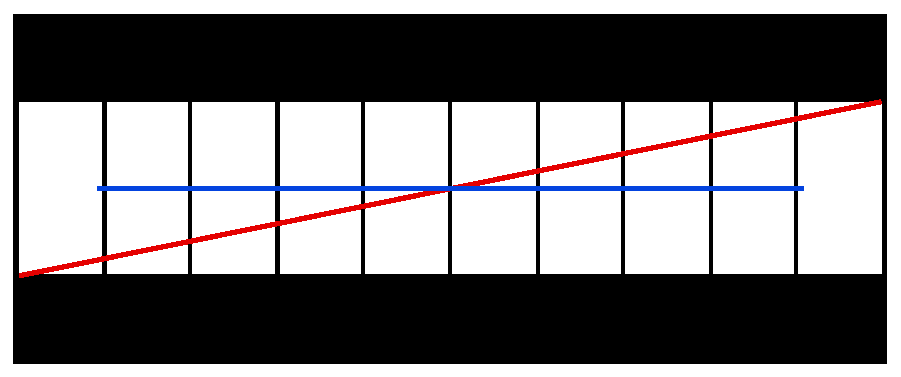
\includegraphics{images/postprocessing/1D_angle}
  \caption{Possible track lengths and angles in a one-dimensional track in AL. The longest, steepest track in red passes through the corners of the most distant pixels, while the shortest, flattest track in blue starts and ends near the nearest edges of the outermost pixels.}
  \label{fig:1D_angle}
\end{figure}

In formulas: A track along an AL line has an angle $\theta$ of

\begin{equation}
  \theta = 0^{\circ} \pm \tan^{-1} \left( \frac{{h_\mathrm{AC}}}{w_\mathrm{AL} \times N_\mathrm{AL}} \right)
  \label{eq:1Dtrackang}
\end{equation}

and a length $l$ of

\begin{equation}
  w_\mathrm{AL} \times \left(N_\mathrm{AL}-2\right) \leq l \leq \sqrt{\left( w_\mathrm{AL} \times N_\mathrm{AL} \right)^{2} + \left( h_\mathrm{AC}\right)^{2}},
  \label{eq:1Dtracklen}
\end{equation}

with
\begin{itemize}
  \item $N_\mathrm{AL}$ being the number of binned pixels in AL
  \item $w_\mathrm{AL}$ being the binned pixel width (i.e. in AL direction)
  \item $h_\mathrm{AC}$ being the binned pixel height.
\end{itemize}

This can be calculated analogously for a track along an AC line. For such tracks, we define our output values for the track angle and length as the mean of Equations \ref{eq:1Dtrackang} and \ref{eq:1Dtracklen} respectively. The uncertainty is then half the absolute value of the difference between the two extreme values of these equations.

For tracks that are not aligned with the AL and AC direction, we use a fitting routine to determine $\theta$, which we in turn use to determine $l$. The fitting routine is shown in Figure \ref{fig:2D_fit}.

\begin{figure}
  \centering
  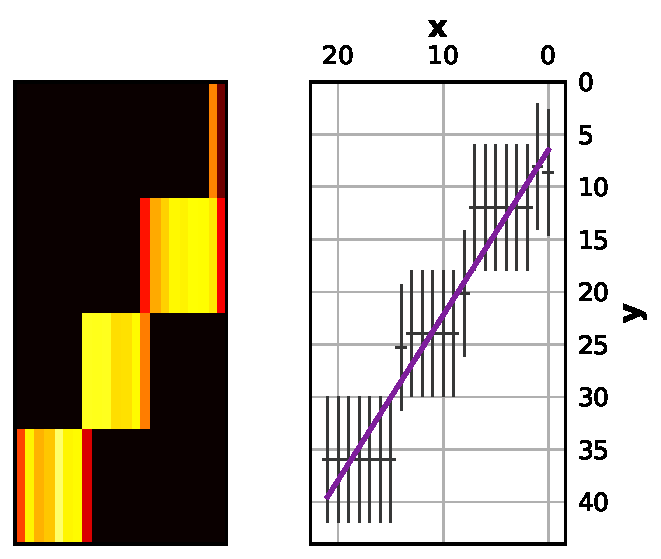
\includegraphics{images/postprocessing/2D_fit}
  \caption{Fitting routine on two-dimensional tracks on the example of a BAM-OBS track. \textit{Left:} Track image, with the pixels scaled to their physical dimension. \textit{Right:} Best fit. The (x, y) pairs have been computed by calculating the center of mass along AC for each AL-line, with the error bars representing the pixel size. The purple line shows the best line fit as determined by orthogonal distance regression.}
  \label{fig:2D_fit}
\end{figure}

For each track image, we first determine the length of the bounding box in binned samples along the AL and AC direction. For each pixel coordinate in the longer axis, we determine the center of mass of the track image values along the shorter axis (e.g. if the image has more pixels in AL, we compute the center of mass along the AC axis for each line). The resulting pairs of values are saved in an $(x,y)$ array, with the x-value denoting the location in AL, the y-value denoting the location in AC multiplied by the factor $f_\mathrm{pix} = 3\times \frac{\mathrm{AC~binning}}{\mathrm{AL~binning}}$. x and y are, as such, in the units of the physical length of a binned AL pixel.

The rationale for using the center of mass is that can better estimate the trajectory of a cosmic if it causes a signal in, for instance, two adjacent pixels in a line -- see the Figure \ref{fig:2D_fit}. 

For each $(x,y)$ pair, we set an uncertainty $(\sigma_x = 0.5, \sigma_y = 0.5 f_\mathrm{pix})$, representing the uncertainty of the detection location due to pixelisation. We then perform a fit of a simple fit to a line equation,

\begin{equation}
  y(x) = m \cdot x + y_0,
\end{equation}

using the \texttt{scipy} implementation of the Orthogonal Distance Regression algorithm \cite{ODR}. This algorithm takes into account the uncertaintes of both $x$ and $y$, providing best fit values and estimations on the standard deviations $\sigma_m$ and $\sigma_{y_o}$ of the slope and offset.

To determine the angle theta and its uncertainty, we utilize the inverse tangent and gaussian error propagation, yielding

\begin{equation}
  \theta = \tan^{-1}\left( m \right), ~~ \sigma_\theta = \frac{1}{m^{2}+1} \sigma_m
\end{equation}

to determine the length of the cosmic, we define the distances $d_x$ and $d_y$ as the difference of x and y between the first and last $(x,y)$ pairs -- if the image has more pixels in AL ($N_\mathrm{AL} \geq N_\mathrm{AC}$), this would be the pairs at the lowest and highest AL, respectively.

To calculate the length, we separate into two cases:
\begin{enumerate}
  \item If $N_\mathrm{AL} \geq N_\mathrm{AC}$, use $d_y = m \cdot d_x$. Then
    \begin{align}
      l &= \sqrt{d_x^{2} + d_y^{2}} = \sqrt{m^{2} + 1} \cdot |d_x|,\\
      \sigma_l^{2} &= \left( m^{2} + 1 \right) \cdot 2 \sigma_x^{2} + \frac{m^{2} d_x^{2}}{m^{2}+1}  \cdot \sigma_m^{2},
    \end{align}
    using Gaussian error propagation for $\sigma_l$.
  \item If $N_\mathrm{AL} < N_\mathrm{AC}$, use $d_x = m^{-1} \cdot d_y$. Then
    \begin{align}
      l &= \sqrt{d_x^{2} + d_y^{2}} = \sqrt{m^{-2} + 1} \cdot |d_y|,\\
      \sigma_l^{2} &= \left( m^{-2} + 1 \right) \cdot 2 \sigma_y^{2} + \frac{d_y^{2}}{m^{4}+m^{6}}  \cdot \sigma_m^{2},
    \end{align}
    using Gaussian error propagation for $\sigma_l$.
\end{enumerate}

the separation into two cases was chosen to avoid numerical unstability, since $d_y$ and $m$ are very small in case 1, while $d_x$ is very small in case 2, and $m$ very large.

\begin{figure}
  \centering
  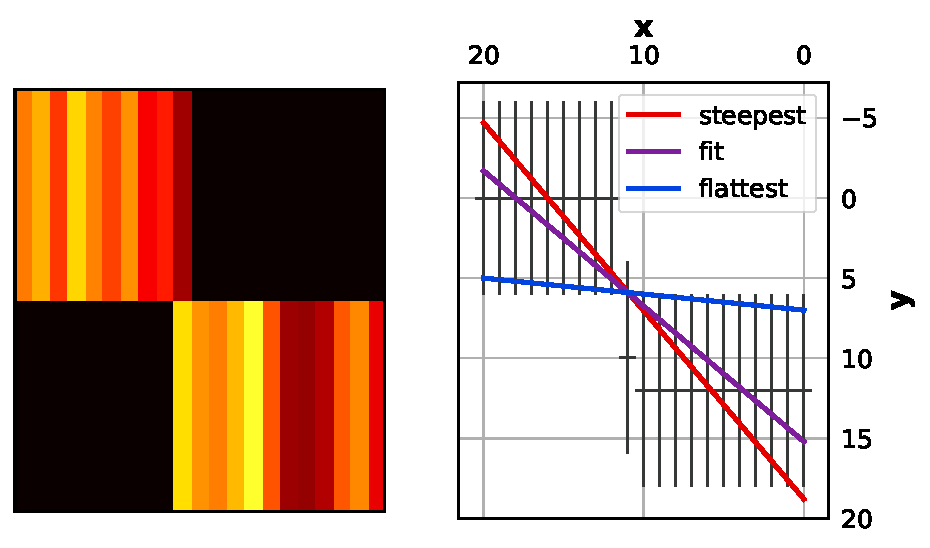
\includegraphics{images/postprocessing/2D_badfit}
  \caption{Issues with fitting tracks whose length in AC or AL is 2. \textit{Left:} Track image, with the pixels scaled to their physical dimension. \textit{Right:} Best line fit and the steepest and flattest plausible associated tracks.}
  \label{fig:2D_badfit}
\end{figure}

This fitting routine was then applied to a subset of all detected tracks in a TrackObs, namely those that
\begin{enumerate}
  \item are two dimensional ($N_\mathrm{AL} > 1$ and $N_\mathrm{AC} > 1$)
  \item contain at least 5 pixels with a signal value
\end{enumerate}

in addition, tracks with $N_AL = 2$ or $N_AC = 2$ must also be significantly longer in their other dimension. This is due to the fact that, as Figure \ref{fig:2D_badfit} outlines, there is a very high uncertainty in the distance crossed along the dimension whose length is two pixels.

To test these analysis routines, we once again used the T.A.R.S. simulator to provide input cosmic rays with known quantites - in this case, the true angle $\theta$ and projected path length $l$. We used the simulator to generate cosmic ray subimages akin to those saved into a track observation. This was done for two cases - one being an SM-like thin chip with a binning of 2 in both AL in AC, the other being a BAM-like thick chip with a binning of 4 in AC and no binning in AL.

In this way, we could predominantly examine the effects of binning and the resulting pixel geometry on the retrieval of the track geometries.

In the case of the SM-like chp, Figure \ref{fig:AngleDist_SM} plots the input angle of the source cosmic versus the measured angle for a long simulation run. Within their accuracies, the measured angles represent the input angles.

\begin{figure}[h]
  \centering
  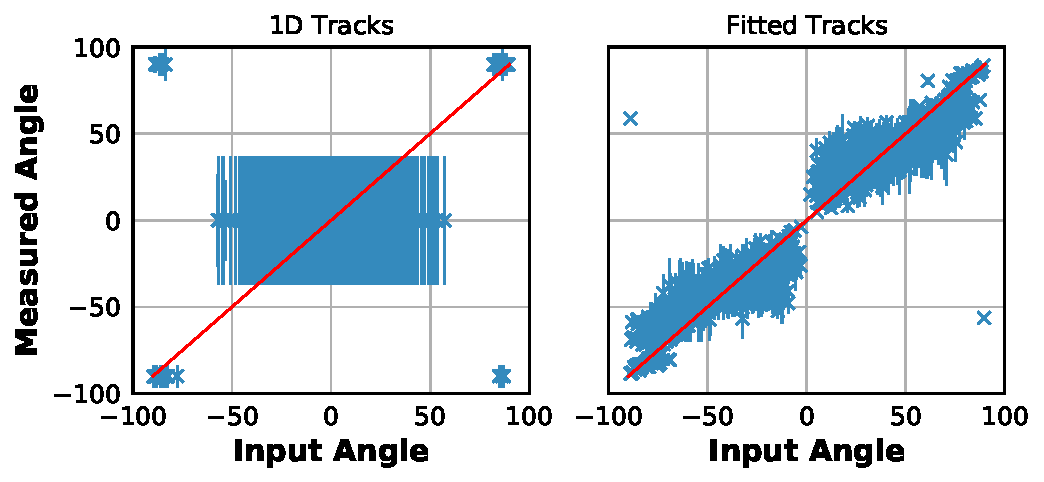
\includegraphics[width=\textwidth]{images/postprocessing/AngleDist_SM}
  \caption{Input angle vs measured angle (in units of degrees) for SM-SIF observations. The error bars represent the uncertainty of the recovered angles, the red diagonal represents the optimal values. The results for one-dimensional and fitted tracks are in the left and right panel, respectively.}
  \label{fig:AngleDist_SM}
\end{figure}

This is better illustrated in Fig. \ref{fig:AngleErr_SM}, which shows histograms of the difference between measured and input angles, normalized by the calculated uncertainties. Here we see that while the fitted cosmics fall well into a Gaussian, the one-dimensional tracks show a bi-modal distribution, where track angles are either systematically under- or over-estimated. Examining Fig. \ref{fig:AngleDist_SM}, these cosmics appear to be those with very large input angles that are nonetheless seen at $\theta = 0^\circ$.

\begin{figure}[h]
  \centering
  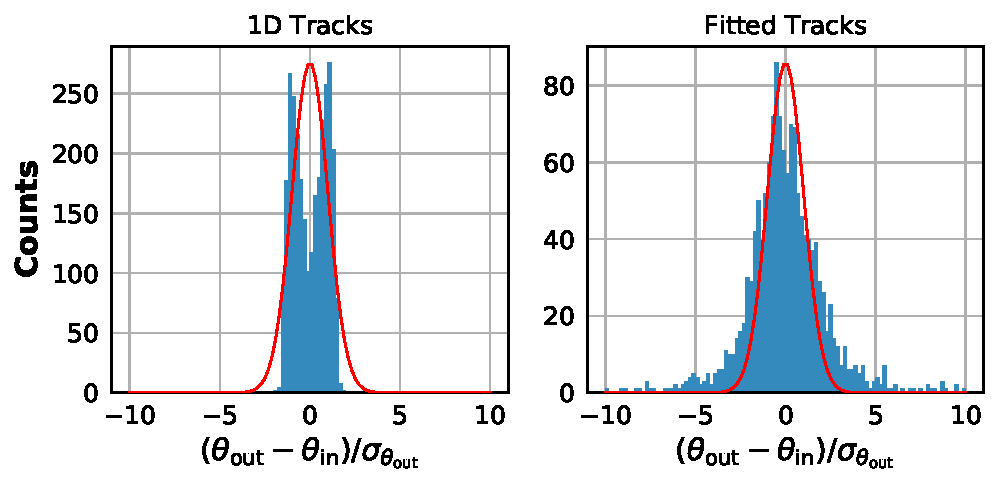
\includegraphics[width=\textwidth]{images/postprocessing/AngleErr_SM}
  \caption{Histograms for the difference of the output angle to the input angle in SM-SIF observations, normalized by the calculated angle uncertainty. The left and right panel show the values for one-dimensional and fitted tracks, respectively. The red curves represent Gaussians with a standard deviation of 1.}
  \label{fig:AngleErr_SM}
\end{figure}

Figure \ref{fig:LenErr_SM} shows similar histograms for the error in the measured track length. These are within the ranges expected by their uncertainty, with a slight systematic overestimation in both indicated by the offset of the maximum from 0.

\begin{figure}[h]
  \centering
  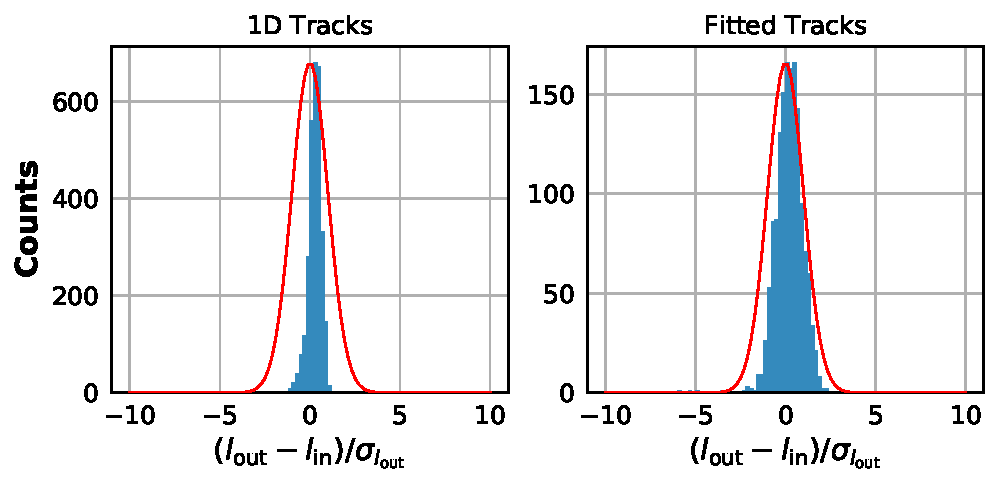
\includegraphics[width=\textwidth]{images/postprocessing/LenErr_SM}
  \caption{Histograms for the difference of the output track length to the input track length in SM-SIF observations, normalized by the calculated length uncertainty. The left and right panel show the values for one-dimensional and fitted tracks, respectively. The red curves represent Gaussians with a standard deviation of 1.}
  \label{fig:LenErr_SM}
\end{figure}

The same analysis for the BAM-like chip shows different systematics. As Figure \ref{fig:AngleDist_BAM} shows, a population of the fitted tracks with $|\theta| \leq 60^{\circ}$ is redistributed to $|\theta| \approx \pm 60^{\circ}$. This is most likely due to the pixel geometry making these tracks appear to have similar angles.

\begin{figure}[h]
  \centering
  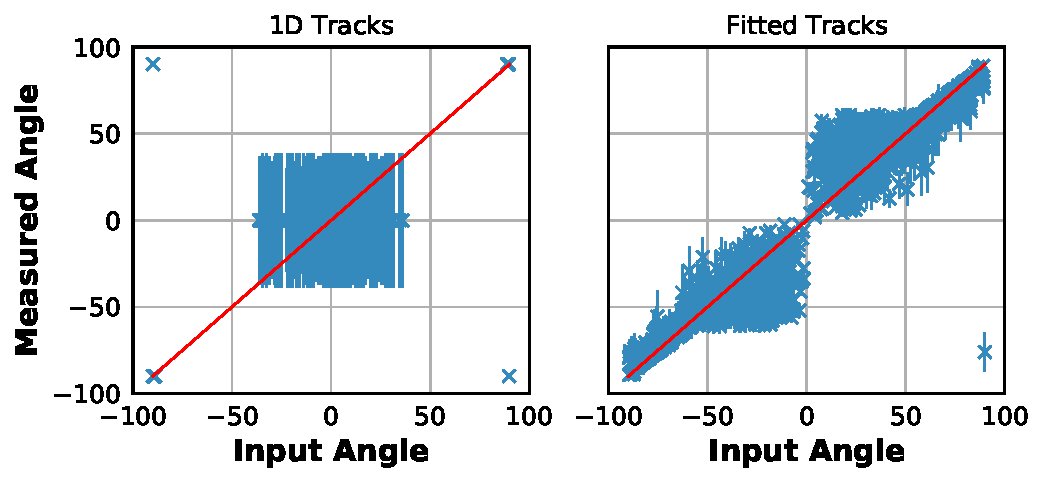
\includegraphics[width=\textwidth]{images/postprocessing/AngleDist_BAM}
  \caption{Input angle vs measured angle (in units of degrees) for BAM-OBS and BAM-SIF observations, as in Fig. \ref{fig:AngleDist_SM}.} 
  \label{fig:AngleDist_BAM}
\end{figure}

The error histograms of the measured angles (Fig \ref{fig:AngleErr_BAM}) shows that while the one-dimensional tracks are all correct within the limits of their uncertainty, the fitted tracks contain some outliers with respect to the bell curve - these are the same cosmics that are mistakenly redistributed to higher angles.

\begin{figure}[h]
  \centering
  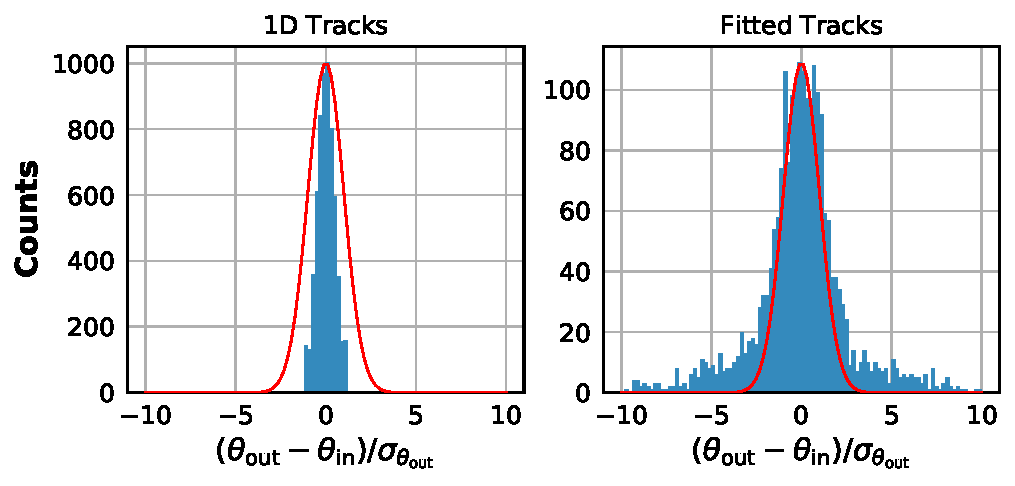
\includegraphics[width=\textwidth]{images/postprocessing/AngleErr_BAM}
  \caption{Histograms for the difference of the output angle to the input angle in BAM-OBS and BAM-SIF observations, as in Fig. \ref{fig:AngleErr_SM}.}
  \label{fig:AngleErr_BAM}
\end{figure}

The measured lengths, plotted for the BAM-like chip in Figure \ref{fig:LenErr_BAM} are once again correctly estimated, with a trend towards an overestimation of the length.

\begin{figure}[h]
  \centering
  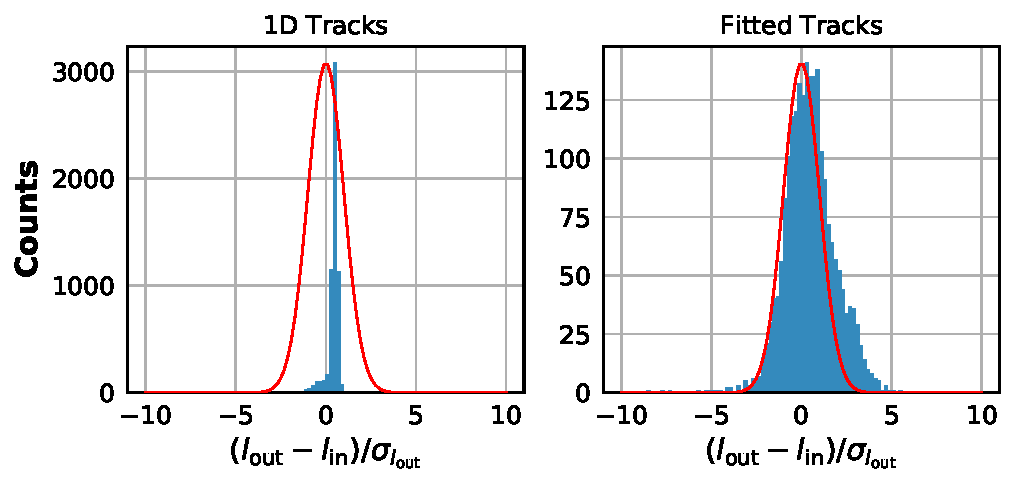
\includegraphics[width=\textwidth]{images/postprocessing/LenErr_BAM}
  \caption{Histograms for the difference of the output track length to the input track length in BAM-OBS and BAM-SIF observations, as in Fig. \ref{fig:LenErr_SM}.}
  \label{fig:LenErr_BAM}
\end{figure}




\subsubsection{Edge Tracks}

Users may not want to use tracks that are located at the edges of a readout window, as the detection does not contain the full energy dumped by the cosmic on the CCD, leading to artificially low energies.  We mark these tracks, applying a flag whenever one or more edges of the bounding box of a track is located on the edge of the input image.


\subsubsection{Post-Processing Pipeline}

\section{Data Model}
\label{sec:datamodel}

This data model is composed of entities {\it CosmicObservation} which are described in full detail in the following subsection.

\subsection{Main Dataset Description}
\label{sec:CosObsModel}

\textbf{Entity Name}:  \textit{CosmicObservation}
\newline
\newline
\textbf{Entity Description}:  A table of cosmic ray (prompt particle event) detections from any of the analyzed Gaia CCDs 
\newline
\newline


\textbf{Entity Header}:
\newline
\begin{table}[!h]
\centering
\resizebox{\textwidth}{!}{\begin{tabular}{|l|l|l|l|}
\hline
{\textit{\textbf{Name}}} & {\textit{\textbf{Description}}} & {\textit{\textbf{Unit}}} & {\textit{\textbf{Type}}} \\ \hline
SOURCE & Descriptor of the type of source observation & NA & String \\ \hline
CCD\_ROW & CCD row of the source chip & NA & Short \\ \hline
FOV & FOV of the source chip & NA & Short \\ \hline
ACQTIME & Source acquisition time & OBMT & Integer \\ \hline
ACQDATE & Source acquisition time & UTC & String \\ \hline
SRC\_AL & AL-dimension of the source image  & pixels & Short \\ \hline
SRC\_AC & AC-dimension of the source image  & pixels & Short \\ \hline
MASKPIX & Number of masked pixels in the source image & pixels & Short \\ \hline
FLUX & Estimated particle flux & particles\,cm$^{-2}$\,s$^{-1}$ & Float \\ \hline
FLUX\_ERR & Poisson Uncertainty of estimated particle flux & particles\,cm$^{-2}$\,s$^{-1}$ & Float \\ \hline
\end{tabular}}
\caption{Event detection table header version \dmVersion}
\end{table}


\textbf{Entity Columns}:
\newline
\begin{table}[!h]
\centering
\resizebox{\textwidth}{!}{\begin{tabular}{|l|l|l|l|}
\hline
{\textit{\textbf{Name}}} & {\textit{\textbf{Description}}} & {\textit{\textbf{Unit}}} & {\textit{\textbf{Type}}} \\ \hline
LOC\_AL & The start position of the event in the AL direction & pixels & Short \\ \hline
LOC\_AC & The start position of the event in the AC direction & pixels & Short \\ \hline
DIM\_AL & Event track dimension in AL & pixels & Short \\ \hline
DIM\_AC & Event track dimension in AC & pixels & Short \\ \hline
TRACK\_NPIX& Number of detected pixels & pixels & Short \\ \hline
TRACK\_EN & Event track total energy  & electrons & Integer \\ \hline
TRACK\_EN\_ERR & Uncertainty in the event track total energy  & electrons & Integer \\ \hline
TRACK\_TRUNCATED & Is the event truncated by start/end of CCD physical area & NA & Boolean \\ \hline
GEOMETRY\_VALID & Is the track geometry (following rows LEN, THETA) applicable?  & NA & Boolean \\ \hline
TRACK\_LEN & Estimated incident particle track length (if applicable) & $\mu$m & Float \\ \hline
TRACK\_LEN\_ERR & Uncertainty in the estimated incident particle track length (if applicable) & $\mu$m & Float \\ \hline
TRACK\_THETA & Estimated incident particle impact angle (if applicable) & deg & Float \\ \hline
TRACK\_THETA\_ERR & Uncertainty in the estimated incident particle impact angle (if applicable) & deg & Float \\ \hline
\end{tabular}}
\caption{Event detection table version \dmVersion}
\end{table}

\subsection{Derived Dataset Description}
\label{sec:FluxModel}
We provide additional files listing just the measured flux per observation.

\subsection{Auxillary Datasets Description}
\label{sec:AuxModel}
\subsubsection{Spacecraft Spin Phase}
\subsubsection{Spacecraft Location}

\section{Persistence Considerations}
\label{sec:persist}
\subsection{Persistence Method(s)}

We should describe here the proposed persistence methods (different alternatives file system based or database), with pros and cons.

\subsection{Size Estimations}

Catalog size estimation is a function of :
\begin{enumerate}
\item The technology used for the generation of this catalog. 
\item The persistence format or system used for storage.
\end{enumerate}

Detection algorithms have been developed and written in Python and the default persistence method adopted is TBD. This results in the following estimations.
\newline
\newline
\textbf{Note:} the following estimations are applicable to catalog version : \dmVersion  
\newline
\newline

Assuming an average event rate (in the absence of solar activity) of : 5 events/s , the average volume of the catalog per spacecraft revolution is : x bytes. Since Gaia performs 4 full revs on it's spin axis every 24 hrs, the average catalog volume per 24 hrs is : y bytes. This needs then to be multiplied by the total nb of mission days covered by the corresponding version of the catalog. 

\subsection{Long Term Preservation}

\section{Quality Control Metrics}
\label{sec:metrics}
Every run of the batch processing cosmic ray detection algorithms shall generate a new version of the catalog. The corresponding version of the catalog will be quality control checked prior to it's official release.

\subsection{Internal Consistency Checks}

\subsection{External Consistency Checks}

\section{Catalog Release Mechanism}
\label{sec:release}
\subsection{Catalog Version Generation}

The proposed catalog versioning scheme is as follows: \newline\newline  \textit{vN.m} \newline\newline where 

\begin{itemize}
\item \textit{N} is a \textit{major} version of the catalog, only updated due to schema updates (i.e, new attributes added or modifications to existing attributes).
\item \textit{m} is a \textit{minor} version of the catalog updated when a new batch processing is performed \textbf{after} algorithmic or software updates. 
\item executions of a new batch processing with no software or algorithm updates but over an increased mission time range result in the increment of the \textit{minor} version of the catalog.

\end{itemize}

Every new version of the catalog (major or minor) will be quality control checked prior to it's official release, according to the criteria described in section~\ref{sec:metrics}.

\subsection{Release Mechanism and Notification to Users}

This is TBD.


\begin{thebibliography}{9}
\bibitem{GAIA-CA-SP-ARI-BAS-003} U. Bastian \emph{Reference Systems, Conventions And Notations for Gaia}.
\bibitem{GAIA-DE-TN-ESAC-RKO-033} R. Kohley \emph{Cosmic rays on BAM CCDs data delivery note}.
\bibitem{Dokkum_cosmics} P. G. van Dokkum \emph{Cosmic-Ray Rejection by Laplacian Edge Detection}.
\bibitem{astroscrappy} C. McCully \emph{Astro-SCRAPPY: The Speedy Cosmic Ray Annihilation Package in Python}, \url{https://github.com/astropy/astroscrappy}.
\bibitem{TARS} Lionel Garcia et al. \emph{Tools for Astronomical Radiation Simulations}
\bibitem{ODR} P. T. Boggs and J. E. Rogers, \emph{Orthogonal Distance Regression}, in ``Statistical analysis of measurement error models and applications: proceedings of the AMS-IMS-SIAM joint summer research conference held June 10-16, 1989,'' Contemporary Mathematics, vol. 112, pg. 186, 1990.


\end{thebibliography}

\end{document}
